\documentclass[10pt,letterpaper]{article} 
\usepackage{cogsci} 
\usepackage{pslatex} 
\usepackage{apacite}
\usepackage{graphicx}
\usepackage{pdfsync}


\title{Preschoolers infer contrast from adjectives if they can access lexical alternatives}

\author{{\large \bf Alexandra Horowitz} \\ \texttt{ahorowit@stanford.edu}\\ Department of Psychology \\ Stanford University \\ 
\And {\large \bf Michael C. Frank} \\ \texttt{mcfrank@stanford.edu} \\ Department of Psychology \\ Stanford University \\ }

\begin{document}

\maketitle

\begin{abstract} 

When speakers use modified noun phrases (e.g. ``long book''), they provide information not only about a salient feature of a single item (i.e. that this book is long), but also about implicit contrasts with possible alternatives (i.e. books can probably vary by length, and some may be short).  We investigate the development of preschoolers' abilities to detect implicit contrasts from speakers' use of adjectives in order to make inferences about category membership of novel items.  In Experiment 1, we found that adults and preschoolers by age 3.5 can make contrast inferences from modifier use in a supportive frame.  In Experiment 2, we reduced the cues to contrast and found adults still inferred implied contrast from adjective use alone, but preschoolers did not.  To test whether increasing accessibility of contrasting adjectives (e.g. `short' for `long') would increase contrast inferences, in Experiment 3 we introduced preschoolers to a training book with opposite pairs prior to the task.  Only older 4-year-olds were able to reliably make contrast inferences and only after the pairs training, suggesting that increasing children's access to alternatives may boost their ability to infer contrast from adjectives alone.  Altogether, our results indicate that preschoolers show increasing sensitivity to the pragmatic implications of speakers' word choices. 

{Keywords:} Pragmatics; adjectives; language development. 
\end{abstract}

\section{Introduction}

A challenge for children learning language is not only to learn the explicit meanings conveyed by semantic content, but also to pick up on available, but implicit, information.  For example, if I refer to ``my youngest sister", a listener can learn not only that I have a younger sister (explicit), but also that the word \emph{youngest} conveys that I have more than one younger sister (implicit).  Thus, speakers can provide underlying information about unstated information through their word choices.  The goal of of our present work was to investigate children's sensitivity to this kind of implicit information conveyed through speakers' lexical decisions. 

%From as young as 18 months, children show some forms of pragmatic reasoning about information provided by speakers.  The principle of contrast \cite{clark1987} describes how children can build on their knowledge of explicit content to form inferences about speakers' intended meaning in what would otherwise be perceived as ambiguous contexts.  For example, if a child is presented with a familiar object (e.g. a spoon) and a novel object (e.g. a spatula) and asked to ``pass the spatula", the child can use the principle of contrast to reason that she already knows a spoon is called a ``spoon", so if the speaker had meant spoon he would have said so.  Therefore ``spatula" must refer to the novel object \cite{clark1990, diesendruck2001, diesendruck2005, gathercole1989}. This suggests that from early on, children are able to apply both their knowledge of explicit information about the world with implicit cues to speakers' likely intended meaning in order to make inferences about novel content. These findings give evidence that young children can consider the implications of the words speakers choose to use, and form inferences depending on these outcomes. 

Although children accumulate impressive vocabularies by kindergarten, children at this age still show surprising difficulties in forming pragmatic inferences about familiar words in conversations.  For example, although adults use word choice to compute scalar implicatures (e.g. that ``some of the horses jumped over the fence implies that some \emph{but not all} of the horses jumped, or else and informative speaker should have used ``all" \cite{grice1975}), 5- to 6-year-olds, accept a semantic overlap such that ``some" can mean some \emph{and possibly all} \cite<e.g.>{papafragou2003, noveck2000}.  Thus, adults show sensitivity to word choice along a lexical scales, though children find it challenging to make the same inferences until fairly late in development.

%the case study of scalar implicatures indicates that 5- to 6-year-olds, and sometimes children even older,  accept that ``some of the horses jumped over the fence" can refer to both a scene in which a subset of the horses jumped over the fence (compatible with adults' interpretation), and a scene in which all of the horses jumped over the fence (incompatible with adults' interpretation) \cite<e.g.>{papafragou2003, noveck2000}.  In other words, adults process terms along a lexical scale as holding mutually exclusive meaning: when all of the horses jumped over the fence, the strongest way to describe this would be to use ``all".  Because we assume that speakers have the Gricean goal of being informative \cite{grice1975}, their choice to use ``some" implies that the stronger alternative ``all" could not be used, and thus infer that only a subset of the horses jumped over the fence.  Thus, where adults compute implicatures from speakers' choices to use a particular item along a lexical scale, children find it challenging to make the same inferences until fairly late in development. \textbf{CUT MORE HERE?}

Why do we see missed inferential opportunities despite children's familiarity with these words? We argue that, unlike some earlier-emerging forms of pragmatic inference involving reference disambiguation in social contexts \cite<e.g.>{clark1990, diesendruck2001, akhtar1996}, computing scalar implicature requires components of reasoning that are importantly distinct.  In order to form a pragmatic inference, a listener must (1) consider the set of alternative utterances the speaker could have made, but chose not to, and (2) generate the belief states that likely correspond with the speakers' lexical choices in contrast to alternative choices.  A critical difference between reference disambiguation and implicature tasks, though both based on inferences about speakers' lexical choices, is their provision of alternatives; in reference selection tasks, children have direct access to alternatives because they are visually present (i.e. naming the familiar or unfamiliar item), but in scalar implicature tasks, children must come up with other possible descriptive choices on their own. 

Barner and colleagues \cite<e.g.>{barner2011, brooks2013} have proposed a \emph{linguistic alternatives hypothesis} to explain children's performance in scalar implicature tasks; children can compute implicatures \emph{only if} they recognize what relevant lexical alternatives compete with the word choice selected.  They find that children can form inferences about implications of word use from mastered scales (e.g. numbers) and from fully comprehended descriptions (e.g. ``the cat and the cow are sleeping" vs. ``only the cat and the cow are sleeping"), but their failure to compute implicatures from weak quantifiers (e.g. ``some of the animals are sleeping") indicates that they do not understand that \emph{some} and \emph{all} are competitors along the same lexical scale.  We extend this hypothesis further to investigate whether access to linguistic alternatives may help explain children's performance in other types of pragmatic tasks.  

In our previous work \cite{horowitz2012}, we investigated preschoolers' inferences about implicit dimensions of contrast from adjective use.  For example, if I describe a novel item as ``tall", it's likely that others may vary by height, but if I instead described it as ``red", it's likely that others may vary by color.  We found that older 4-year-olds (age 4.5 -- 5.0) were able to form contrast inferences from both color and size terms, but that younger 4-year-olds (age 4.0 -- 4.5) exhibited a bias to match by color regardless of the adjective used.  We propose that our results may be related to children's abilities to access the appropriate linguistic alternatives; although children are familiar with color naming, children may not recognize color use as contrastive because there is not a particular implied contrast item per se (``red" implies that others may be ``not red", but not that another item will necessarily be a specific color, e.g. ``blue").  In this manner, our task may have been difficult for younger children because they did not appreciate that adjective use implies a relevant contrast dimension.  In our current work, we extend our task to include familiar scalar contrasts children have more experience with in order to determine whether their performance depends on their knowledge of implied linguistic alternatives.  We replaced color terms with familiar feature opposites (e.g. wet--dry and dirty--clean) to examine whether children succeed when they are very familiar with the lexical contrasts being used.

In this paper, we outline preschoolers' and adults' contrast inferences from familiar scalar opposites across three experiments using a similar paradigm.  In the task, participants heard a modified noun phrase to describe a novel shape and were then asked to select what they thought another category member looked like: either one that matched by the property referenced by the modifier, or one that contrasted along the referenced property dimension.  In Experiment 1, we found that adults (Experiment 1a) and preschoolers by age 3.5 (Experiment 1b) reliably selected the shape that contrasted by the referenced property.  In Experiment 2, adults' performance was sustained when framing cues supporting contrast were reduced (Experiment 2a), but preschoolers were at chance at inferring implicit contrast information from adjective use alone (Experiment 2b).  In Experiment 3, we read a book of opposites with preschoolers before undergoing the task from Experiment 2b, and found that this increased older children's contrast judgments.  Overall, our results give support that children's performance in pragmatics tasks relates to their ability to consider alternatives; children formed contrast inferences in our tasks that provided supportive framing and a reminder of opposites, but had difficulty recognizing the opportunity for inference when from adjective use alone. 


\section{Experiment 1a: Adults} 

We first wanted to confirm adults' sensitivity to implicit contrast information conveyed though adjective use before investigating children's performance.  We described a novel shape in a contrastive framing referencing either a feature or size adjective, and asked adults to infer what other category members look like.  If adults detect an implied dimension of contrast from adjective use, they should infer that other shapes are likely to vary along that property.  This is precisely what we found.  



%we aimed to increase the salience of the adjective referenced with the support of contrastive framing (i.e. ``This is a special kind of [tibu]...").  If adults detect an implied dimension of contrast from adjective use, they should infer that other shapes are likely to vary along that property.  This is precisely what we found.  


%We extended a previous paradigm \cite{horowitz2012} designed to isolate adjective use as the only informative cue to relevant properties of novel category membership.  We introduced participants to set of three pictures: an exemplar shape, and two shapes that each differ from the exemplar by a single property, either feature or size (Figure \ref{fig:demo}).  We describe the exemplar using either a feature or size adjective, and ask adults to predict what other category members look like.  With the goal of modifying the task for children, we aimed to increase the salience of the adjective referenced with the support of contrastive framing (i.e. ``This is a special kind of [tibu]...").  If adults detect an implied dimension of contrast from adjective use, they should infer that other shapes are likely to vary along that property.  This is precisely what we found.  
\subsection{Methods}

\subsubsection{Participants}

A planned sample of 128 adult participants was recruited from Amazon's Mechanical Turk online crowd-sourcing service.  Three subjects were excluded for failing to complete the task. All participants reported that they were native speakers of English and were informed that the task was designed for children.  

\subsubsection{Stimuli}

Participants were presented with cartoon images of items from outer space. They participated in a single test trial featuring a set of three pictures: one referenced exemplar shape and two test shapes, one that differed from the exemplar shape only by a feature, and another that differed from the exemplar shape only by size (Figure \ref{fig:demo}).  Participants were randomly assigned to one of four sets of test shapes.  


\begin{figure}[t] 
  \begin{center} 
  \vspace{-1in}
    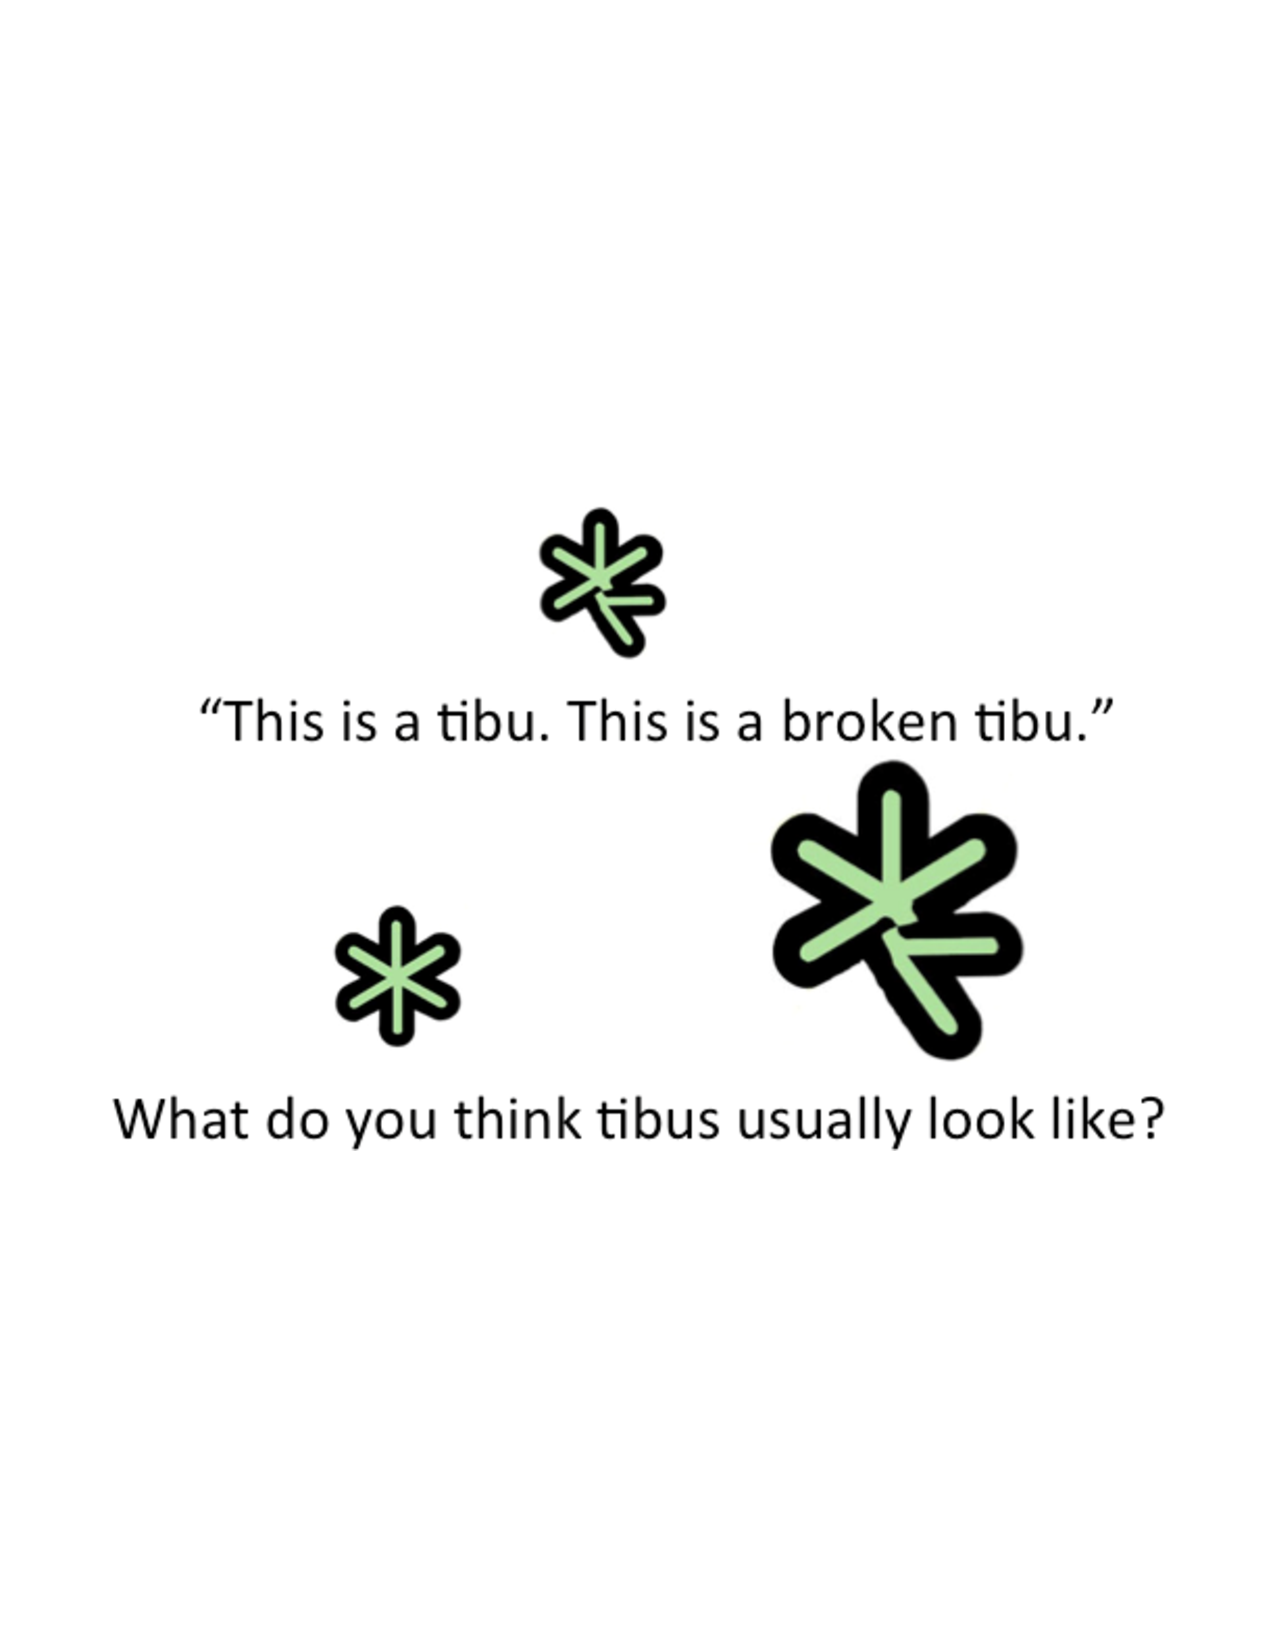
\includegraphics[width=3in]{figures/demo.pdf} 
   % \vspace{-1in}
   \vspace{-1in}
    \caption{\label{fig:demo} Example trial shape set.  In the contrastive language conditions (Experiments 1a and 1b), the first sentence was modified from ``This is a tibu" to ``This is a special kind of tibu."  All other expressions remained the same. }
    %Participants saw a set of three novel shapes: a training exemplar (e.g. small broken) followed by a test set containing one shape that differed only by a state feature (e.g. small unbroken), and one that differed only by size (e.g. big broken). Participants were told that a character uttered an expression modified by an adjective (feature or size), and asked to predict which test exemplar represented what that kind of shape usually looked like.  In the contrastive language conditions (Experiments 1a and 1b), the first sentence altered from ``This is a tibu" to ``This is a special kind of tibu."  All other expressions remained the same. } 
  \end{center} 
  % \vspace{-2.0ex} 
\end{figure}
	


%They were also randomly assigned to one of two conditions: in the \emph {contrastive language} condition, the labeled shape was introduced with language cues supporting contrast inferences (i.e. ``This is a \textbf{special kind of} [tibu]. This is a [broken tibu].")  In the adjective only condition, the labeled shape was introduced simply as ``This is a [tibu]. This is a [broken tibu]".

 
%Participants read a story online in which a cartoon character, Allen the Alien, introduced them to a novel shape from outer space.  They participated in a single test trial featuring a forced choice between two similar shapes: one that differed from the first only by size, and another that differed from the first only by feature (Figure \ref{fig:demo}).  Participants were randomly assigned to one of four sets of test shapes (which constitute each of the four trials in Experiments 2 and 3 with children), and either a \emph{contrastive language} or \emph{adjective only} condition.  In the contrastive language condition, Allen the Alien provided supportive cues to implicit contrast by stating ``This is a \textbf{special kind of} [tibu]. This is a [broken tibu]."  In the adjective only condition, he simply introduced the shape as ``This is a [tibu]. This is a [broken tibu]".

\subsubsection{Procedures}

Participants read a story online in which a cartoon character, Allen the Alien, introduced them to a novel shape from outer space and said something about it, e.g. ``This is a special kind of tibu.  This is a [broken] tibu." Half of participants were presented with a feature adjective (e.g. ``broken") and half were presented with a size adjective (e.g. ``small").  They were then shown the two test shapes and asked, ``What do you think [tibus] usually look like?", and prompted to select one of the two images.  We measured the proportion of participants who selected the picture that contrasted with the named property. 


\subsection{Results and Discussion}

Responses were coded as correct if participants selected the shape that differed along the referenced dimension.  In other words, we considered a response to be a correct contrast judgement if the participant selected the shape that differed by feature in feature adjective trials (e.g. heard ``broken" and selected the shape that was unbroken), and differed by size in size adjective trials (e.g. heard ``small" and selected the shape that was big).  

Participants selected the contrasting dimension at nearly identical rates and more often than chance for both adjective types ($p < .001$ in exact binomial tests for feature and size terms).  Our results indicate that participants used the adjective referenced to make inferences about properties of novel category members, suggesting that adjectives are informative indicators of relevant property information to adults.  They were able to consider the labeled property in order to infer that other novel category members are likely to differ along the referenced dimension.  Our adult participants expertly detected implicit contrast information from adjective word choice, and we next turned to investigate children's sensitivity to these available cues.  

%, and performance did not differ significantly across the contrastive language and adjective only conditions ($\chi^2(3) = 4$, $p = .26$, Figure \ref{fig:res5}).

%Adults were sensitive to adjective use in our task, even when no other linguistic cues were provided to imply a contrast inference.  These results suggest that adjectives are informative indicators of relevant property information to adults; they were able to consider the labeled property in order to infer that other novel category members are likely to differ along the referenced dimension.  Our adult participants expertly implicit contrast information from adjective word choice, and we next turned to investigate children's sensitivity to these available cues.  
	
\begin{figure}[t] 
  \begin{center} 
    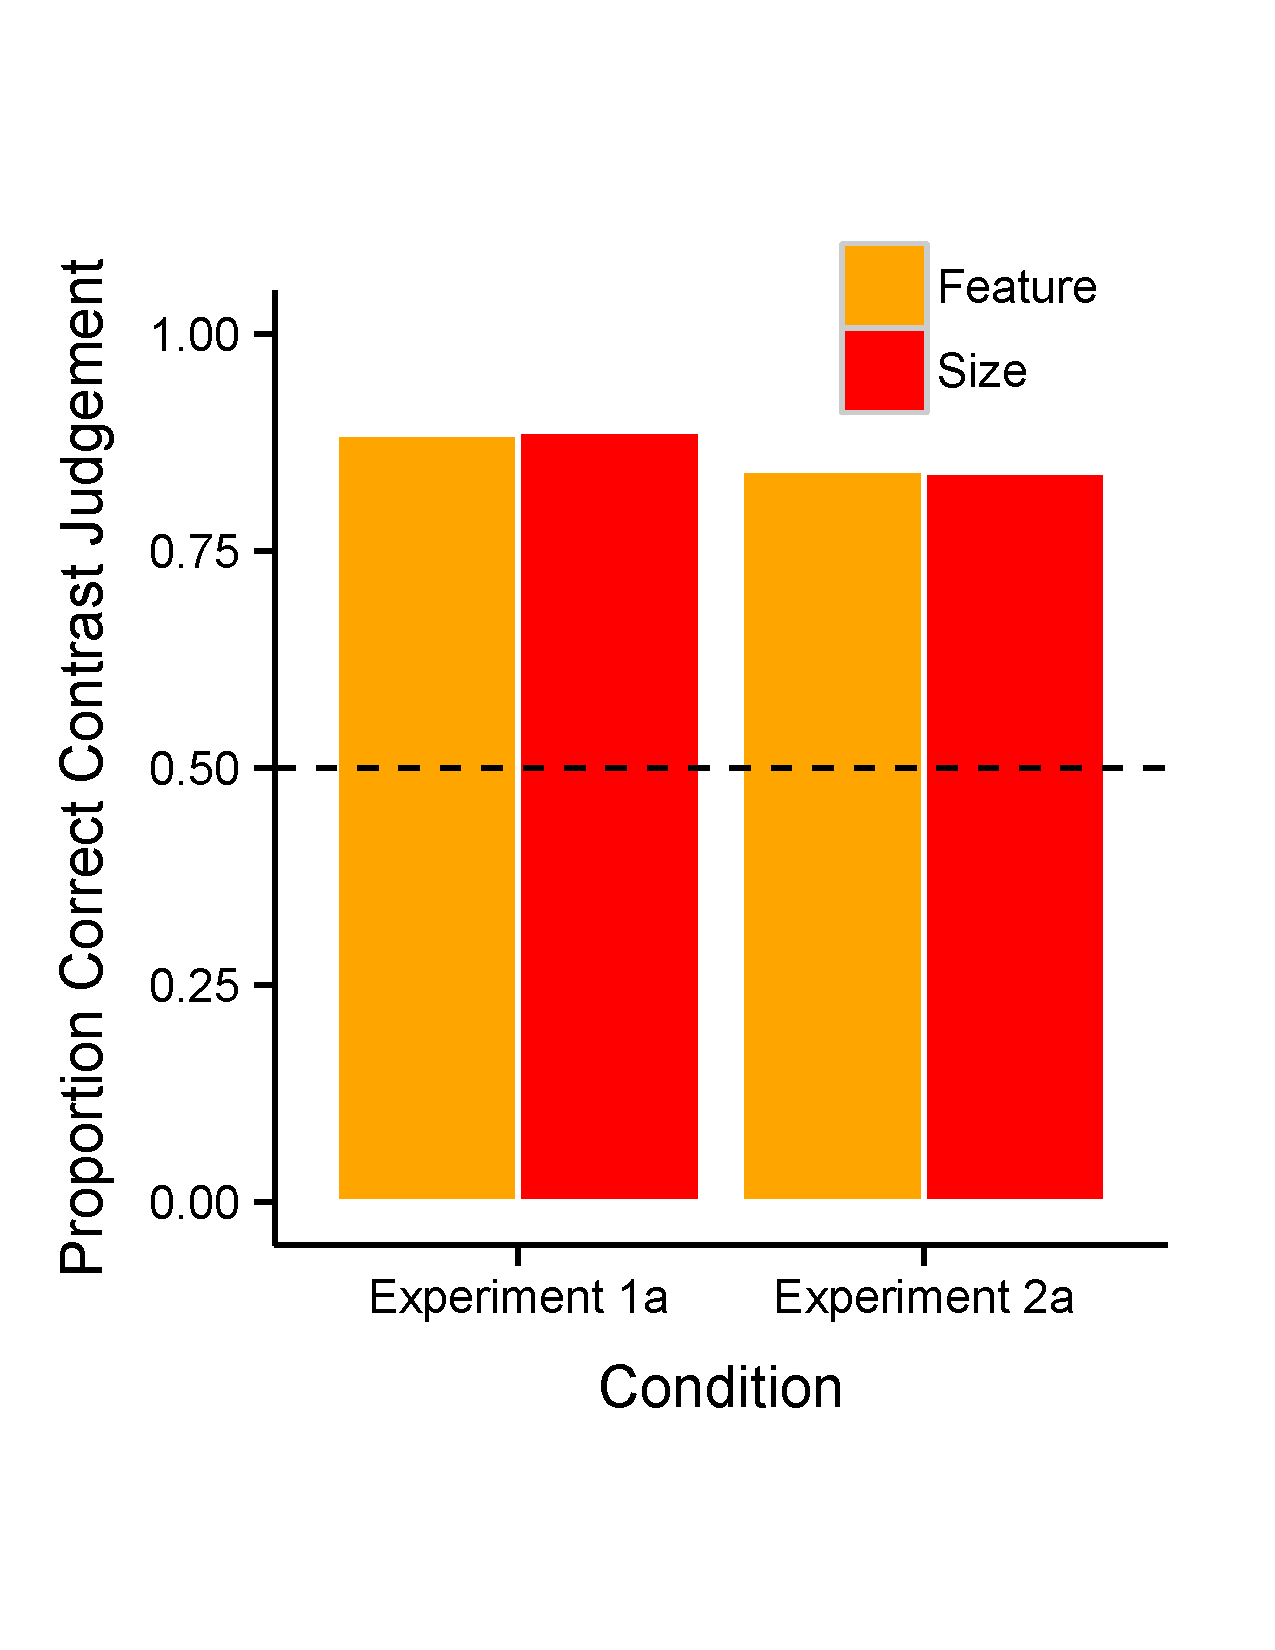
\includegraphics[width=3in]{figures/adults2.pdf} 
    \caption{\label{fig:res5} Adults' mean proportion correct performance in Experiments 1a and 2a. Feature trials are plotted in yellow and size trials in red.The dashed line represents chance (0.5). }
    %Error bars represent 95\% confidence intervals.} 
  \end{center} 
  % \vspace{-2.0ex} 
\end{figure}	




%\begin{figure}[t] 
%  \begin{center} 
 %   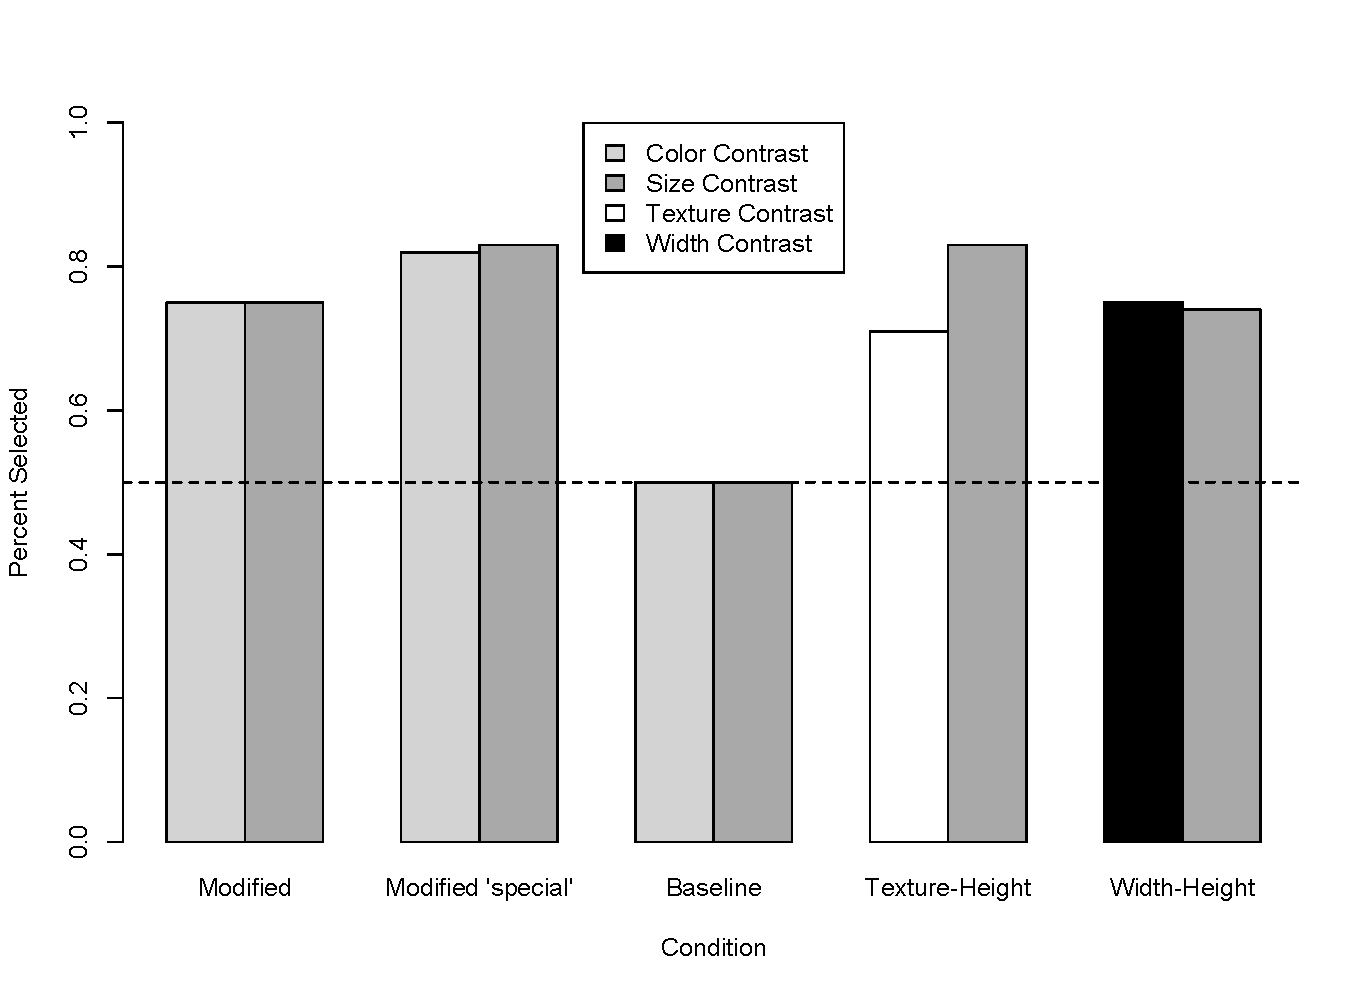
\includegraphics[width=3.6in]{figures/adults_all2.pdf} 
%    \caption{\label{fig:res2} Mean percent correct performance across Experiments 1-3 with adult %participants. The dashed line represents chance (50\%). Adults performed significantly above %chance for all trials other than the baseline.} 
%  \end{center} 
%  % \vspace{-2.0ex} 
%\end{figure}





\section{Experiment 1b: Children} 

In Experiment 1b, we modified the task into a four trial storybook for children.  Because the feature and size opposites used are some of the earliest learned, we used a wide sample of 3- to 4-year-olds, broken into half-year age brackets.    If children are sensitive to implicit contrasts conveyed through adjectives, they should select the image contrasting along the referenced dimension.  If they do not recognize variable property cues from adjective, then they should select at random or choose the image that matches (rather than contrasts with) the stated adjective. 

\subsection{Methods}

\subsubsection{Participants}

We recruited 96 four-year-old children from the Bing Nursery School at Stanford University and the San Jose Children's Discovery Museum.  Twenty-four children were recruited to each of four age groups: age 3.0 -- 3.5 (M = 3;3), age 3.5 -- 4.0 (M = 3;8), age 4.0 -- 4.5 (M = 4;3), and age 4.5 -- 5.0 (M = 4;8).  About half of each age group was recruited from each location.

\subsubsection{Stimuli}

We adapted the task for adults into a physical book the experimenter read with children.  Each child participated in two training trials with pictures of familiar objects before undergoing four test trials.  The test trials featured each of the individual test sets used with adults, presented in one of two orders.  For each child, two of the test trials referenced a feature adjective, and two of the test trials referenced a size adjective.  Test image sets were presented in one of two orders, and adjective type and image presentation were counterbalanced across participants. 


\subsubsection{Procedures}

Children were tested individually in a quiet room at the nursery school or museum.  The experimenter sat next to the children at a table and read a printed storybook with the clipart images from Experiment 1a. Children were introduced to the character Allen the Alien and completed two training trials with common images to familiarize them with the task (%e.g. ``This is a special kind of milk. This is chocolate milk.  What does milk usually look like?").  
If children did not select the correct image during a familiarization trial, they were prompted the correct image was chosen.
%Children who did not spontaneously select the correct image during training were prompted until they did so.  

The training trials were followed by four test trials.  In each test trial, the child was first shown an image of a single exemplar shape and heard Allen say something about it, e.g. ``This is a special kind of tibu. This is a broken tibu."  The experimenter then uncovered two test pictures, one that differed but by the exemplar only by feature, and one that differed from the exemplar only by size.  Children were asked, ``What do you think tibus usually look like? What do most tibus look like?" and prompted to point to one of the test images.  The experimenter averted her eyes as children indicated their responses. 
%and provided no explicit feedback.  
%For two test trials children heard a reference to a feature adjective, and for two test trial they heard a reference to a size adjective.  Test image sets were presented in one of two orders, and adjective type and image presentation were counterbalanced across participants. 
Children also participated in a posttest following the test trials in order to demonstrate their knowledge of the adjectives used in the study.  Test sessions took about 10 minutes to complete and were video recorded.  

\begin{figure}[t] 
  \begin{center} 
    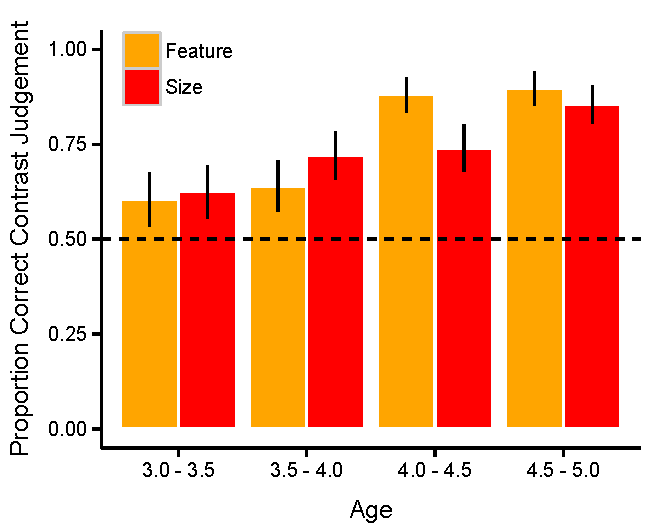
\includegraphics[width=3.5in]{figures/experiment1bResults.pdf} 
    \caption{\label{fig:kids1} Preschoolers' mean proportion correct performance in Experiment 1b. Yellow bars depict feature adjective trials and red bars. The dashed line represents chance (0.5). Error bars represent standard error.}
    %95\% confidence intervals.} 
  \end{center} 
  % \vspace{-2.0ex} 
\end{figure}	




\subsection{Results and Discussion}

Preschoolers in our task did show sensitivity to implied contrast dimensions conveyed through adjective use.  Only the youngest children in our sample (ages 3 -- 3.5 years) did not reliably select the adjective contrast reliably about chance.  By age 3. 5, children were able to infer category membership from word choice cues by choosing the image contrasting by feature when a feature term was referenced and the image contrasting by size when a size term was referenced, and performance increase with age (Figure \ref{fig:kids1}).


We analyzed our results using a logic mixed model, predicting correct responses as an interaction between age and contrast type with random effects of participant and alien type.  Children increasingly made more correct contrast judgments with age ($\beta = 1.51$, $p < .0001$).
% There was a significant effect of age, such that children increasingly made more correct contrast judgments with age ($\beta = 1.51$, $p < .0001$).   
  There was no significant effect of contrast type (feature vs. size adjectives), and there was no interaction between age and contrast type, suggesting that participants across ages did not differ in their responses to different property types.  Overall, these analyses show that children demonstrate an increasing sensitivity to implicit contrast information from adjectives.  


 %Exact binomial tests for each adjective type per binned age group indicate that the youngest children respond at chance levels (, but that children 3.5 -- 4.0 responded  

The posttest data reveal that children overwhelmingly were  knowledgeable about the terms we used in our task.  Correct identifications averaged 90\% ages 3.0 -- 3.5, 95\% ages 3.5 -- 4.0, 96\% ages 4.0 -- 4.5, and 98\% ages 4.5 -- 5.0.  These scores indicate that children's comprehension is improving with age, but that even the youngest children in the sample overall were knowledgeable of the terms used. 


%To ensure that performance differences were not due to unfamiliarity with the color and size terms, we ran a posttest with a subset of children for each age group (n=13 younger, n=12 older). Younger children produced the correct size term over 80\% and color terms 95\% of the time.  Older children's production was 94\% for size and 99\% for color. These data suggest that younger children's lower performance on color trials was not a result of not knowing their color words.


%\textbf{We captured this pattern with a second logit mixed model, this time predicting choice of color-matching target as a function of trial type (including baseline), age group, and their interaction. In this analysis, we saw that younger children had a significant bias for color ($\beta = 1.32$, $p = .004$), and a trend towards differential responding in color trials ($\beta = -.83$, $p = .09$). There was a significant coefficient on older children's bias, indicating more size responding ($\beta = -2.02$, $p = .002$), as well as a significant interaction for size trials, indicating success in overcoming this baseline effect ($\beta = 1.76$, $p = .04$), but only for size trials. Thus, both groups showed some bias in their responding, but older 4s were better able to overcome that bias---at least for size---and make inferences about why a particular adjective was produced. }

Our results from Experiment 1b indicate that preschoolers by age 3.5 were sensitive to the adjective provided as an indicator of implicit contrast.  Although each of the two test images were equally similar to the first because each differed by only a single property, children avoided selecting the property match (i.e. selecting the picture that was the \emph{same} property as the one referenced, e.g. hearing ``broken" and selection the other broken image) and instead selected the image \emph{differing} along the referenced dimension (e.g. hearing ``broken" and selecting the picture that was unbroken. This suggests that preschoolers are able to consider the pragmatic implications of word choice in our task to infer that the adjective selection conveys information about a relevant property \emph{dimension} of interest: remarking on a novel shape's size implies that size may vary across category members, but reference to a feature highlights that the feature property may vary by individual.  

We next turned to investigate the robustness of these inferences.  If listeners are sensitive to adjective choice generally, then they should be able to maintain inferences about implicit contrasts even without contrastive language framing cues.  If their recognition of the informativeness of adjective choice is more fragile, they may rely on the addition of supportive linguistic cues guiding a contrastive interpretation. 


%\textbf{REMINDER OF COUNTERINTUITIVE: NOT ONLY LEARNING BAOUT SINGLE INSTANCE< BUT INFERRING MORE GENRALLY}


\section{Experiment 2a: Adults} 

%In Experiment 1, we designed the cues to contrast to be as strong as possible in order to examine whether preschoolers can make use of adjective information to infer implicit contrast information.  We found that by age 3.5 years, children were able to reliably select the property contrast to the adjective referenced.  
%At least in contexts supporting cues to contrast, young children can use feature and size descriptors to learn not only about the present exemplar, but also to infer a relevant dimension of contrast for other category members.  

In order to test the extent of adults' sensitivity to implicit contrasts, we reran Experiment 1a with the framing cues to contrast removed.  We found that adults were just as likely to form contrast inferences from adjective use alone as they were with the supportive framing. 
%We next wanted to investigate listeners' sensitivity to word choice when other framing cues to contrast were removed.  In Experiment 2, we remove the supportive framing of ``special kind of..." in order to isolate adjective use as the only available cue to contrast.  If listeners are perceptive of implicit dimensions of contrast conveyed by adjectives, their performance should match that of Experiment 1. If adjectives alone are not salient enough to carry relevant property information, then contrast inferences should decrease with this minimal framing.  We begin again by testing adults before examining children's performance, and find that they form contrast inferences from adjective use both with and without the additional support of contrastive framing. 

\subsection{Methods}

\subsubsection{Participants}

A new planned sample of 128 adult participants were recruited from Amazon's Mechanical Turk online crowd-sourcing service.  Two subjects were excluded for failing to complete the task. All participants reported that they were native speakers of English and were informed that the task was designed for children.  

\subsubsection{Stimuli}

Stimuli were identical to Experiment 1a. 

\subsubsection{Procedures}

Procedures were identical to Experiment 1a with the exception that the referential phrase was reduced by removing the phrase ``special kind of" so that listeners heard only ``This is a [tibu]. This is a [broken tibu]."   This subtle change allowed us to examine listeners' inferences from adjective use without drawing attention to it via the framing.  

\subsection{Results and Discussion}

As above, we measured the proportion of correct contrast judgments for which participants selected the test picture that differed along the referenced property dimension.  Adults performance was ($p < .001$ in exact binomial tests for feature and size terms) and did not differ by adjective type.  They showed only a slight decrease in performance in this adjective only framing from the contrastive language framing in Experiment 1a.  These results indicate that adjective use in our task is a strong indicator of relevant property information of novel category members to adults.  Their nearly equal performance across Experiment 1a and 2a suggests that adjectives provided salient cues to implicit contrast dimensions on their own without the necessity of additional semantic support. 

\section{Experiment 2b: Children} 

We reran Experiment 1b with the contrastive framing removed in order to examine children's sensitivity to adjective use alone. Although even 3.5-year-olds reliably inferred contrasts from properties referenced in Experiment 1b, even children a full year older still had difficulty succeeding in the present experiment without the support of contrastive framing.  

\subsection{Methods}

\subsubsection{Participants}

A new sample of \textbf{38} children from Bing Nursery School.  Because of the presumed increased difficulty of this task, we began by matching to the older age groups in the previous sample: 4.0- to 4.5-year-olds \textbf{(M = 4;3)} and 4.5- to 5.0-year-olds \textbf{(M = 4;8)}.

\subsubsection{Stimuli}

Stimuli were identical to Experiment 1b. 

\subsubsection{Procedures}

Procedures were identical to Experiment 1b with the exception that the referential phrase was minimized by removing the phrase ``special kind of" to reduce contrast cues other than the adjective.  Instead, they heard only ``This is a [tibu]. This is a [broken tibu]," isolating the adjective as the only available indicator of category membership.

\subsection{Results and Discussion}

Unlike preschoolers' increasing ability to make contrast selections from adjective use in Experiment 1b, they were only at chance when the contrastive language framing was removed.  Older 4s showed a significant feature contrast bias ($p < .001$ in exact binomial text) suggesting that children may infer default states for familiar state descriptors (e.g. ``fixed" instead of ``broken"), but no other responses differed from chance.  We analyzed our results using a logic mixed model, predicting correct responses as an interaction between age and contrast type with random effects of participant and alien type, and we found no significant effects or interaction.  Although adults remained attentive to implicit contrast information provided by modifier selection in both the contrastive language and adjective only referential framings, children appeared to rely on additional linguistic cues to guide their contrast judgements.  



%Preschoolers' in Experiment 2b did not appear sensitive to the the informativeness of property reference when the adjective was provided as the only marker of category information. 


%\textbf{STILL COLLECTING DATA/RUNNING ANALYSES}

One explanation for the discrepancy in children's performance from Experiment 1b to Experiment 2b is that they require more information than an adjective alone to cue a contrast inference.  Although adults can conjure implicit contrast information from individual word choices, children may rely on the combination of informative lexical selections with the addition of supportive linguistic framing.  

%In other words, children may understand that modified noun phrases convey 
Another reason for children's shift in contrast inferences across experiments is not that they necessarily need contrast intentions to be explicitly conveyed, but rather that they require an awareness of what lexical alternatives \emph{could} have been used in place of the ones chosen.  Extending the linguistic alternatives hypothesis to our current task, children's contrast inferences may not relate to framing per se, but rather their access to scalar alternatives.  We investigated this idea in Experiment 3 but increasing the availability of property contrasts. 


%Barner and colleagues \cite<e.g.>{barner2011} propose that children's variable performance in other pragmatic task such as computing scalar implicatures can be explained by their access to linguist alternatives; preschoolers succeed in implicature tasks about word choice only when they understand what relevant alternative choices were opted over in favor of the selected descriptor.  In terms of the current task, children's conferences may not relate to framing per se, but rather their access to scalar alternatives.  We investigated this idea in Experiment 3 but increasing the availability of property contrasts. 
%r relevant alternatives could have  In other words, children's difficulty in Experiment 2b may be caused by an inability to consider relevant lexical competitors (e.g. scalar opposites) instead of framing cues to intention.  


\begin{figure}[t] 
  \begin{center} 
    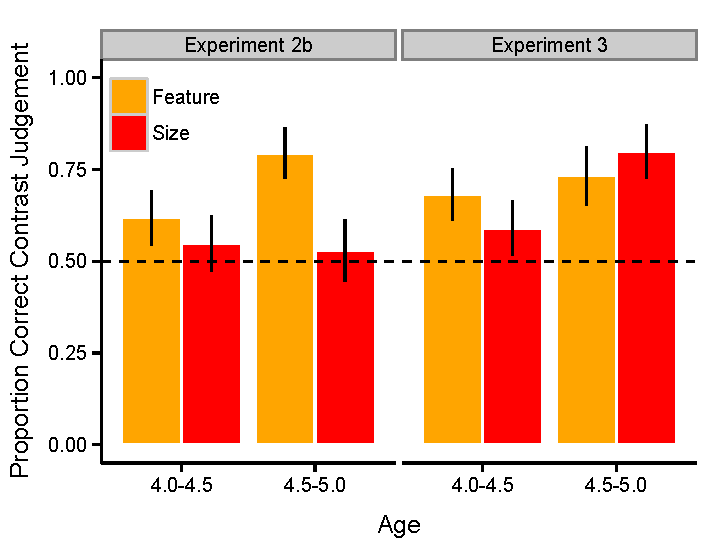
\includegraphics[width=3.7in]{figures/results_expt2b&3_n75.pdf} 
    \caption{\label{fig:kids2} Preschoolers' mean proportion correct performance in Experiments 2b and 3.  Feature adjective trials are plotted in yellow and size trials in red.
   % Yellow bars represent feature adjective trials, and red bars represent size adjective trials
%    proportion of feature contrast selections in feature adjective trials, and the red bars represent the proportion of size contrast selections in size adjective trials.  
The dashed line represents chance (0.5). Error bars show standard error.}
  \end{center} 
  % \vspace{-2.0ex} 
\end{figure}

\section{Experiment 3} 



%Although children succeeded in forming contrast inferences from adjective with in the contrastive language framing (Experiment 1b), they had difficulty when the adjective was provided on its own without other cues to contrast (Experiment 2b). 

In Experiment 3, we provide a test of the linguistic alternatives theory by increasing preschoolers' access to the relevant lexical alternatives.  Before the experimental procedure, the experimenter read a seemingly unrelated book featuring the opposites referenced in the test trials (see Figure \ref{fig:training}).  This exposure to linguistic alternatives boosted older 4-year-olds' contrast selections. 

\subsection{Methods}

\subsubsection{Participants}

A new sample of \textbf{37} children from Bing Nursery School. Participants were grouped into two age groups: 4.0- to 4.5-year-olds \textbf{(M = 4;3)} and 4.5- to 5.0-year-olds \textbf{(M = 4;8)}.

\subsubsection{Stimuli}

Stimuli were identical to Experiment 1b and 2b with the addition of a separate training book.  The training book consisted of clip art pairs of familiar images depicting the size and feature scalar contrasts portrayed in the test book (e.g. \emph{small/big, broken/fixed}.  Opposite pairs were labeled consecutively to maximize the salience of a given contrast dimension. 

\subsubsection{Procedures}

Children were told that they would be reading two books for the session.  The procedure was identical to that of Experiment 2b with the addition of an opposites training book immediately preceding the test book. The experimenter read the training book with children, labeling the picture in neutral way on each page (e.g. ``This is a small teddybear. This is a big teddybear").  Although the properties used in both books were the same, no child explicitly noted any connection between the books. 

\subsection{Results and Discussion}

Increasing preschoolers' access to relevant linguistic alternatives helped older 4s select property contrasts for both feature and size adjectives.  These results suggest that supporting children's abilities to bring relevant alternatives in mind plays a strong role in their pragmatic inferences. Beyond relying on rich semantic framing cues to intended meaning, which is not always available in natural speech, reminding children of different types of modifiers increases their likelihood of forming contrast inferences from adjectives alone. 

Older children selected the contrast property for both feature and size terms more often than chance ($p < .001$ and $p < .05$ respectively in exact binomial tests) and younger children for feature terms ($p < .05$ in exact binomial test), though younger children's performance did not differ across feature and size trials.  A logic mixed model predicting correct responses as an interaction between age and contrast type with random effects of participant and alien type, revealed no significant effects or interaction, however.

When we combine results with those of Experiment 2b, we find a marginal three-way interaction between experiment, adjective type, and age, such that older children show improved contrast inferences for size only after the opposites book ($\beta = 2.64$, $p =0.08$).  Increased access to lexical alternatives seemed to help older children reliably select the dimension contrast according to the property.  

Our results from Experiment 3 suggest that exposing children to a book of unrelated pictures with scalar alternatives used in our test trials helped older children form contrast inferences from the minimal cue of a modified noun phrase.  We believe that the initial book did not serve to train children to make contrast selections because we did not see a change in performance for the youngest children.  In addition, anecdotally none of the children remarked on any relationship connection between the books, even though they conveyed the same adjective properties.  Instead, we believe that the opposites book served to make the lexical scales more accessible to children so that, at least for the oldest children in our task, they could spontaneously infer implicit contrast information from an adjective produced alone.   

%\vspace

\begin{figure}[t] 
  \begin{center} 
    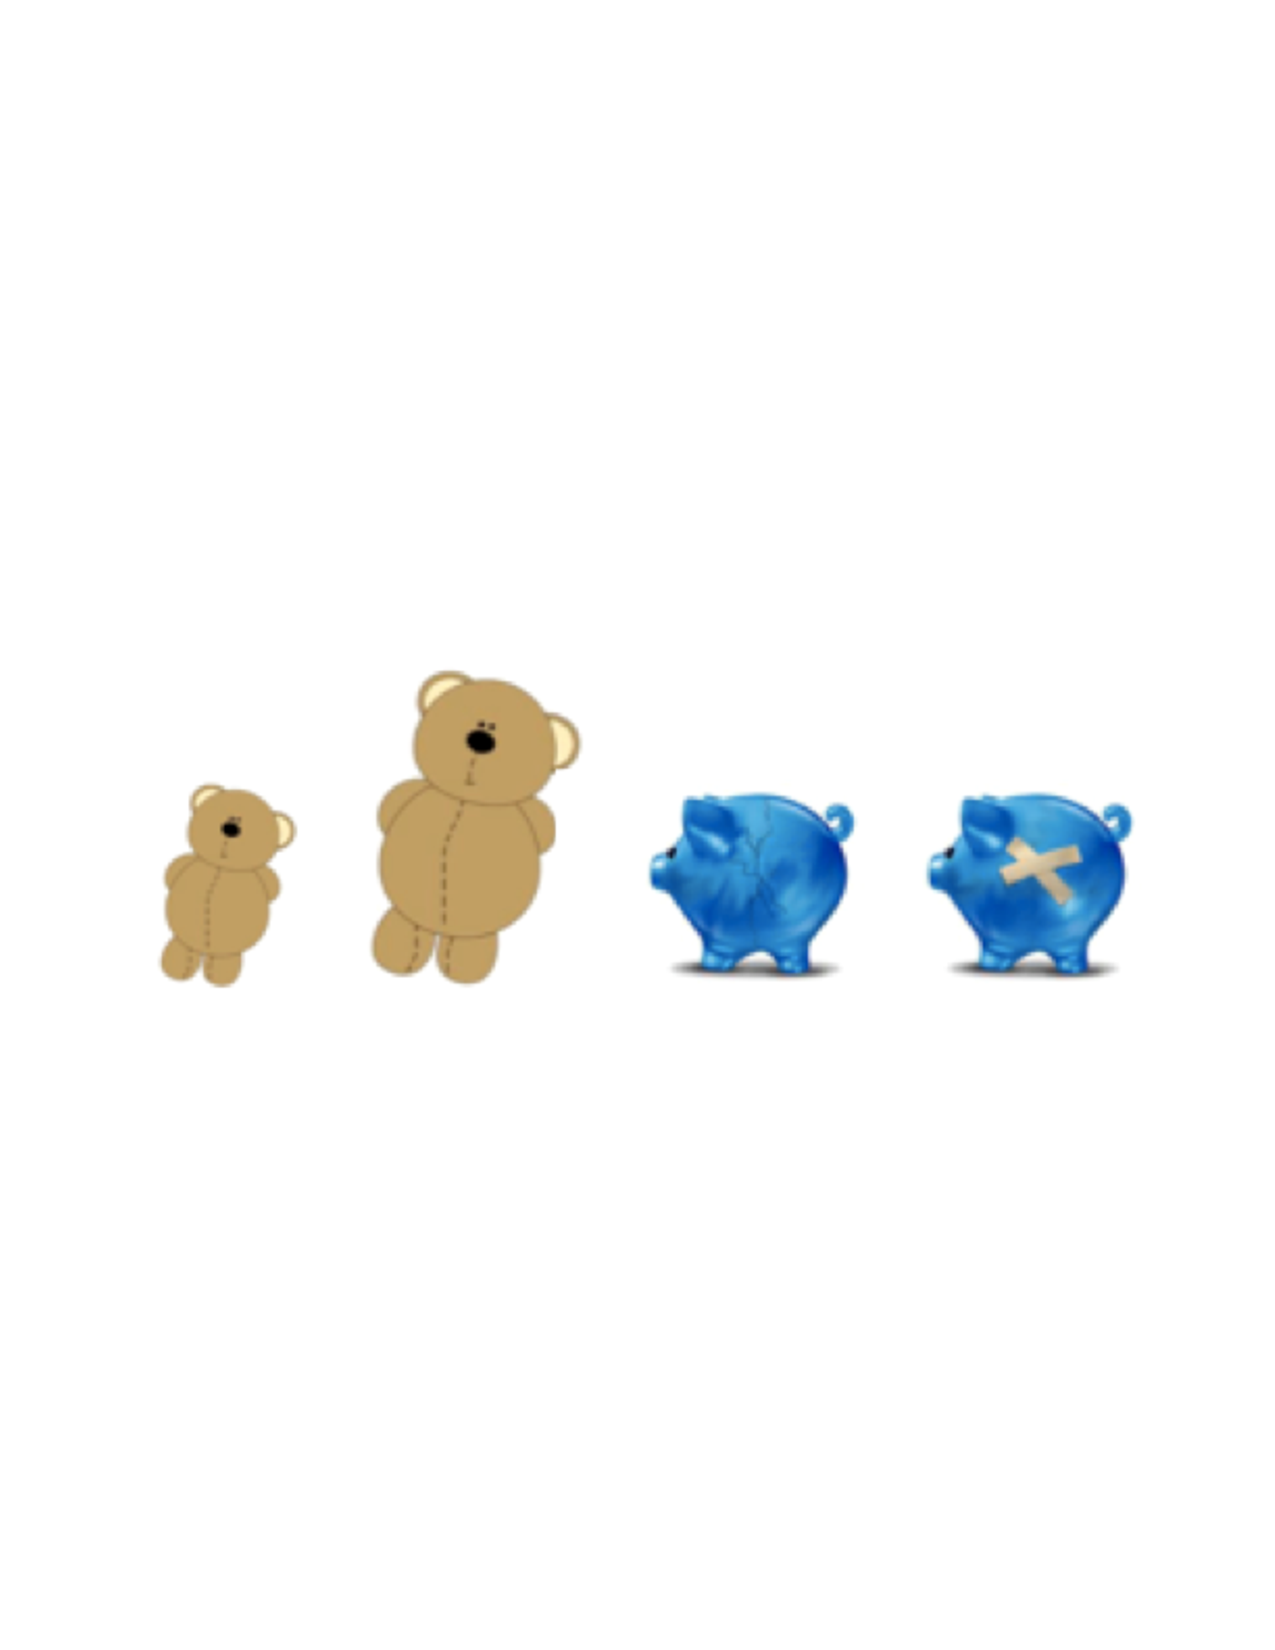
\includegraphics[width=3.5in]{figures/opposites_demo_long.pdf} 
    \vspace{-2in}
    \caption{\label{fig:training} Examples of training pairs used in Experiment 3.  Top row depicts a size contrast (small -- big) and bottom row a feature contrast (broken -- fixed).}
  \end{center} 
  % \vspace{-2.0ex} 
\end{figure}


% \begin{table} [t]
%   \caption{Coefficient estimates from a generalized liner mixed model predicting performance as an interaction between contrast type (color and size) and age group (younger or older than four-and-a-half). \label{tab:1b} } 
%   \begin{center} 
%     \begin{tabular}{lrrrr} 
%       \hline 
%       \null & Coef. & Std. Error & $z$ &$p(|z|)$\\ 
%       \hline Intercept (4s) & 1.39 & 0.51 & 2.71 & $<$0.01\\ 
%       Contrast & -0.56 & 0.72 & -0.79 & 0.43\\ 
%       Age & -2.06 & 0.71 & -2.92 & $<$0.01\\
%        Contrast x Age & 3.25 & 1.02 & 2/17 &  $<$0.01\\ 
%       \hline 
%     \end{tabular} 
%   \end{center}
%   % \vspace{-2.0ex} 
% \end{table}

%This may reflect the development of general pragmatic capabilities across this age range. 

 \section{General Discussion} 

We set out to investigate whether the linguistic alternatives hypothesis might be applied to pragmatic tasks beyond computing scalar implicatures.  Our results suggest that children's performance in our tasks does seem to be related to their ability to consider relevant lexical alternatives.  In Experiment 1, participants robustly selected the category membership as the image contrasting with the property referenced when supported by contrastive language framing.  In Experiment 2, adults maintained performance but preschoolers were hindered to chance performance when framing was reduced so that the adjective was the only available cue to contrast.  We suggest that children were unable to recognize adjective use on its own as an indicator of implicit contrast information along its referenced property dimension rather than simply a salient descriptor.  In Experiment 3, we helped increase 4-year-olds' access to linguistic alternatives by previewing the task with a book of opposites, and found that this boosted older children's rate of contrast inferences.  

The inferences measured in our task are fairly counterintuitive: a correct contrast judgment requires selecting the property \emph{contrast} instead of the property \emph{match}, although both choices are available in each set.  Our findings that even children as young at age 3.5 can reliably make contrast selections from both size and feature adjectives in supportive contexts demonstrates that young children are sensitive to the pragmatic implications of speakers' word choices.  Their diminished success in the adjective only condition but recovered contrast inferences after the opposites exposure further suggests that the linguistic alternatives hypothesis may explain this pattern of performance; children are able to form pragmatic inferences when they recognize word choice as conveying implicit contrasts with relevant implicit alternatives, but they appear to fail when they are unable to access implied lexical alternatives spontaneously from adjective use alone.  In other words, children can recognize adjective use as conveying information about implicit contrast dimensions, but unlike adults, they may need additional cues supporting these inferences until they gain enough experience to form these inferences on their own. 

The ability to infer implicit information can allow children to learn about the world more efficiently.  When children can recognize implied contrasts conveyed through word choices, they can learn not only about a particular instance (e.g. ``This is a small tibu"), but can also form inferences about additional information conveyed about the speaker's knowledge or perspective of the world from their word choices (e.g. tibus are likely to vary by size).  In order to form these inferences, children may need enough experience with language and particular property comparisons to recognize pragmatic opportunities.  This may explain both why children fail to compute scalar implicatures for weak quantifies and why they failed to form contrast inferences from our previous work featuring color terms.  Opportunities to pick up on informative underlying cues to meaning are constantly conveyed through speech, and children sensitive to these cues by appreciating implicit linguistic alternatives will be able to learn more effectively and efficiently from their interactions. 

%Can adults and children learn from speakers' choice of a particular adjective? Our results suggest that adults are able to infer the general structure of a category based on the words chosen to describe a specific, anomalous example. Children also showed sensitivity to word choice, though we saw developmental differences between ages four and five. Children older than four-and-a-half sometimes succeeded in making inferences based on word choice, while younger children primarily exhibited a color bias. Our corpus analysis suggests that the language adults use with children around this age may mark color as implying a salient, immediate dimension, whereas size was used for a wider variety of functions.  

%The ability to make inferences from speakers' word choices may not only reflect more adult-like comprehension, but may also be an important learning mechanism for children.  The earlier and faster children can go beyond what is stated at face value, the more opportunities they have to gain further knowledge through pragmatic cues. This kind of inference is consistent with work suggesting that pragmatic mechanisms can be used in a variety of different kinds of inferences: for inferring speaker meaning, learning words, and in this case, inferring facts about the world \cite{frank2009}.
% Making these inferences allows greater amounts of information to be exchanged more efficiently.  

%Children who are able to recognize that word choices can convey broader information will have greater opportunities for learning about the world, because they can recognize both what is explicitly stated and implicitly implied. This ability allows children both to learn more from each utterance and to increase learning opportunities by requesting additional information. Although pragmatic inferences are not always easy for children, our results suggest that these inferences may become an important source of background knowledge about the world. 

\section{Acknowledgments}

Special thanks to the staff and families at the Bing Nursery School and the San Jose Children's Discovery Museum.

\bibliographystyle{apacite}

\setlength{\bibleftmargin}{.125in} \setlength{\bibindent}{-\bibleftmargin}

\bibliography{ADJ}

\end{document}

